%% bare_conf.tex
%% V1.3
%% 2007/01/11
%% by Michael Shell
%% See:
%% http://www.michaelshell.org/
%% for current contact information.
%%
%% This is a skeleton file demonstrating the use of IEEEtran.cls
%% (requires IEEEtran.cls version 1.7 or later) with an IEEE conference paper.
%%
%% Support sites:
%% http://www.michaelshell.org/tex/ieeetran/
%% http://www.ctan.org/tex-archive/macros/latex/contrib/IEEEtran/
%% and
%% http://www.ieee.org/

%%*************************************************************************
%% Legal Notice:
%% This code is offered as-is without any warranty either expressed or
%% implied; without even the implied warranty of MERCHANTABILITY or
%% FITNESS FOR A PARTICULAR PURPOSE! 
%% User assumes all risk.
%% In no event shall IEEE or any contributor to this code be liable for
%% any damages or losses, including, but not limited to, incidental,
%% consequential, or any other damages, resulting from the use or misuse
%% of any information contained here.
%%
%% All comments are the opinions of their respective authors and are not
%% necessarily endorsed by the IEEE.
%%
%% This work is distributed under the LaTeX Project Public License (LPPL)
%% ( http://www.latex-project.org/ ) version 1.3, and may be freely used,
%% distributed and modified. A copy of the LPPL, version 1.3, is included
%% in the base LaTeX documentation of all distributions of LaTeX released
%% 2003/12/01 or later.
%% Retain all contribution notices and credits.
%% ** Modified files should be clearly indicated as such, including  **
%% ** renaming them and changing author support contact information. **
%%
%% File list of work: IEEEtran.cls, IEEEtran_HOWTO.pdf, bare_adv.tex,
%%                    bare_conf.tex, bare_jrnl.tex, bare_jrnl_compsoc.tex
%%*************************************************************************

% *** Authors should verify (and, if needed, correct) their LaTeX system  ***
% *** with the testflow diagnostic prior to trusting their LaTeX platform ***
% *** with production work. IEEE's font choices can trigger bugs that do  ***
% *** not appear when using other class files.                            ***
% The testflow support page is at:
% http://www.michaelshell.org/tex/testflow/



% Note that the a4paper option is mainly intended so that authors in
% countries using A4 can easily print to A4 and see how their papers will
% look in print - the typesetting of the document will not typically be
% affected with changes in paper size (but the bottom and side margins will).
% Use the testflow package mentioned above to verify correct handling of
% both paper sizes by the user's LaTeX system.
%
% Also note that the "draftcls" or "draftclsnofoot", not "draft", option
% should be used if it is desired that the figures are to be displayed in
% draft mode.
%
\documentclass[conference]{IEEEtran}
\usepackage[pdftex]{graphicx}
\graphicspath{{images/}}
\DeclareGraphicsExtensions{.pdf,.jpeg,.png}
\usepackage{caption}
\usepackage{subcaption}
\usepackage{subfig}
% Add the compsoc option for Computer Society conferences.
%
% If IEEEtran.cls has not been installed into the LaTeX system files,
% manually specify the path to it like:
% \documentclass[conference]{../sty/IEEEtran}





% Some very useful LaTeX packages include:
% (uncomment the ones you want to load)


% *** MISC UTILITY PACKAGES ***
%
%\usepackage{ifpdf}
% Heiko Oberdiek's ifpdf.sty is very useful if you need conditional
% compilation based on whether the output is pdf or dvi.
% usage:
% \ifpdf
%   % pdf code
% \else
%   % dvi code
% \fi
% The latest version of ifpdf.sty can be obtained from:
% http://www.ctan.org/tex-archive/macros/latex/contrib/oberdiek/
% Also, note that IEEEtran.cls V1.7 and later provides a builtin
% \ifCLASSINFOpdf conditional that works the same way.
% When switching from latex to pdflatex and vice-versa, the compiler may
% have to be run twice to clear warning/error messages.






% *** CITATION PACKAGES ***
%
%\usepackage{cite}
% cite.sty was written by Donald Arseneau
% V1.6 and later of IEEEtran pre-defines the format of the cite.sty package
% \cite{} output to follow that of IEEE. Loading the cite package will
% result in citation numbers being automatically sorted and properly
% "compressed/ranged". e.g., [1], [9], [2], [7], [5], [6] without using
% cite.sty will become [1], [2], [5]--[7], [9] using cite.sty. cite.sty's
% \cite will automatically add leading space, if needed. Use cite.sty's
% noadjust option (cite.sty V3.8 and later) if you want to turn this off.
% cite.sty is already installed on most LaTeX systems. Be sure and use
% version 4.0 (2003-05-27) and later if using hyperref.sty. cite.sty does
% not currently provide for hyperlinked citations.
% The latest version can be obtained at:
% http://www.ctan.org/tex-archive/macros/latex/contrib/cite/
% The documentation is contained in the cite.sty file itself.






% *** GRAPHICS RELATED PACKAGES ***
%
\ifCLASSINFOpdf
  % \usepackage[pdftex]{graphicx}
  % declare the path(s) where your graphic files are
  % \graphicspath{{../pdf/}{../jpeg/}}
  % and their extensions so you won't have to specify these with
  % every instance of \includegraphics
  % \DeclareGraphicsExtensions{.pdf,.jpeg,.png}
\else
  % or other class option (dvipsone, dvipdf, if not using dvips). graphicx
  % will default to the driver specified in the system graphics.cfg if no
  % driver is specified.
  % \usepackage[dvips]{graphicx}
  % declare the path(s) where your graphic files are
  % \graphicspath{{../eps/}}
  % and their extensions so you won't have to specify these with
  % every instance of \includegraphics
  % \DeclareGraphicsExtensions{.eps}
\fi
% graphicx was written by David Carlisle and Sebastian Rahtz. It is
% required if you want graphics, photos, etc. graphicx.sty is already
% installed on most LaTeX systems. The latest version and documentation can
% be obtained at: 
% http://www.ctan.org/tex-archive/macros/latex/required/graphics/
% Another good source of documentation is "Using Imported Graphics in
% LaTeX2e" by Keith Reckdahl which can be found as epslatex.ps or
% epslatex.pdf at: http://www.ctan.org/tex-archive/info/
%
% latex, and pdflatex in dvi mode, support graphics in encapsulated
% postscript (.eps) format. pdflatex in pdf mode supports graphics
% in .pdf, .jpeg, .png and .mps (metapost) formats. Users should ensure
% that all non-photo figures use a vector format (.eps, .pdf, .mps) and
% not a bitmapped formats (.jpeg, .png). IEEE frowns on bitmapped formats
% which can result in "jaggedy"/blurry rendering of lines and letters as
% well as large increases in file sizes.
%
% You can find documentation about the pdfTeX application at:
% http://www.tug.org/applications/pdftex





% *** MATH PACKAGES ***
%
%\usepackage[cmex10]{amsmath}
% A popular package from the American Mathematical Society that provides
% many useful and powerful commands for dealing with mathematics. If using
% it, be sure to load this package with the cmex10 option to ensure that
% only type 1 fonts will utilized at all point sizes. Without this option,
% it is possible that some math symbols, particularly those within
% footnotes, will be rendered in bitmap form which will result in a
% document that can not be IEEE Xplore compliant!
%
% Also, note that the amsmath package sets \interdisplaylinepenalty to 10000
% thus preventing page breaks from occurring within multiline equations. Use:
%\interdisplaylinepenalty=2500
% after loading amsmath to restore such page breaks as IEEEtran.cls normally
% does. amsmath.sty is already installed on most LaTeX systems. The latest
% version and documentation can be obtained at:
% http://www.ctan.org/tex-archive/macros/latex/required/amslatex/math/





% *** SPECIALIZED LIST PACKAGES ***
%
%\usepackage{algorithmic}
% algorithmic.sty was written by Peter Williams and Rogerio Brito.
% This package provides an algorithmic environment fo describing algorithms.
% You can use the algorithmic environment in-text or within a figure
% environment to provide for a floating algorithm. Do NOT use the algorithm
% floating environment provided by algorithm.sty (by the same authors) or
% algorithm2e.sty (by Christophe Fiorio) as IEEE does not use dedicated
% algorithm float types and packages that provide these will not provide
% correct IEEE style captions. The latest version and documentation of
% algorithmic.sty can be obtained at:
% http://www.ctan.org/tex-archive/macros/latex/contrib/algorithms/
% There is also a support site at:
% http://algorithms.berlios.de/index.html
% Also of interest may be the (relatively newer and more customizable)
% algorithmicx.sty package by Szasz Janos:
% http://www.ctan.org/tex-archive/macros/latex/contrib/algorithmicx/




% *** ALIGNMENT PACKAGES ***
%
%\usepackage{array}
% Frank Mittelbach's and David Carlisle's array.sty patches and improves
% the standard LaTeX2e array and tabular environments to provide better
% appearance and additional user controls. As the default LaTeX2e table
% generation code is lacking to the point of almost being broken with
% respect to the quality of the end results, all users are strongly
% advised to use an enhanced (at the very least that provided by array.sty)
% set of table tools. array.sty is already installed on most systems. The
% latest version and documentation can be obtained at:
% http://www.ctan.org/tex-archive/macros/latex/required/tools/


%\usepackage{mdwmath}
%\usepackage{mdwtab}
% Also highly recommended is Mark Wooding's extremely powerful MDW tools,
% especially mdwmath.sty and mdwtab.sty which are used to format equations
% and tables, respectively. The MDWtools set is already installed on most
% LaTeX systems. The lastest version and documentation is available at:
% http://www.ctan.org/tex-archive/macros/latex/contrib/mdwtools/


% IEEEtran contains the IEEEeqnarray family of commands that can be used to
% generate multiline equations as well as matrices, tables, etc., of high
% quality.


%\usepackage{eqparbox}
% Also of notable interest is Scott Pakin's eqparbox package for creating
% (automatically sized) equal width boxes - aka "natural width parboxes".
% Available at:
% http://www.ctan.org/tex-archive/macros/latex/contrib/eqparbox/





% *** SUBFIGURE PACKAGES ***
%\usepackage[tight,footnotesize]{subfigure}
% subfigure.sty was written by Steven Douglas Cochran. This package makes it
% easy to put subfigures in your figures. e.g., "Figure 1a and 1b". For IEEE
% work, it is a good idea to load it with the tight package option to reduce
% the amount of white space around the subfigures. subfigure.sty is already
% installed on most LaTeX systems. The latest version and documentation can
% be obtained at:
% http://www.ctan.org/tex-archive/obsolete/macros/latex/contrib/subfigure/
% subfigure.sty has been superceeded by subfig.sty.



%\usepackage[caption=false]{caption}
%\usepackage[font=footnotesize]{subfig}
% subfig.sty, also written by Steven Douglas Cochran, is the modern
% replacement for subfigure.sty. However, subfig.sty requires and
% automatically loads Axel Sommerfeldt's caption.sty which will override
% IEEEtran.cls handling of captions and this will result in nonIEEE style
% figure/table captions. To prevent this problem, be sure and preload
% caption.sty with its "caption=false" package option. This is will preserve
% IEEEtran.cls handing of captions. Version 1.3 (2005/06/28) and later 
% (recommended due to many improvements over 1.2) of subfig.sty supports
% the caption=false option directly:
%\usepackage[caption=false,font=footnotesize]{subfig}
%
% The latest version and documentation can be obtained at:
% http://www.ctan.org/tex-archive/macros/latex/contrib/subfig/
% The latest version and documentation of caption.sty can be obtained at:
% http://www.ctan.org/tex-archive/macros/latex/contrib/caption/




% *** FLOAT PACKAGES ***
%
%\usepackage{fixltx2e}
% fixltx2e, the successor to the earlier fix2col.sty, was written by
% Frank Mittelbach and David Carlisle. This package corrects a few problems
% in the LaTeX2e kernel, the most notable of which is that in current
% LaTeX2e releases, the ordering of single and double column floats is not
% guaranteed to be preserved. Thus, an unpatched LaTeX2e can allow a
% single column figure to be placed prior to an earlier double column
% figure. The latest version and documentation can be found at:
% http://www.ctan.org/tex-archive/macros/latex/base/



%\usepackage{stfloats}
% stfloats.sty was written by Sigitas Tolusis. This package gives LaTeX2e
% the ability to do double column floats at the bottom of the page as well
% as the top. (e.g., "\begin{figure*}[!b]" is not normally possible in
% LaTeX2e). It also provides a command:
%\fnbelowfloat
% to enable the placement of footnotes below bottom floats (the standard
% LaTeX2e kernel puts them above bottom floats). This is an invasive package
% which rewrites many portions of the LaTeX2e float routines. It may not work
% with other packages that modify the LaTeX2e float routines. The latest
% version and documentation can be obtained at:
% http://www.ctan.org/tex-archive/macros/latex/contrib/sttools/
% Documentation is contained in the stfloats.sty comments as well as in the
% presfull.pdf file. Do not use the stfloats baselinefloat ability as IEEE
% does not allow \baselineskip to stretch. Authors submitting work to the
% IEEE should note that IEEE rarely uses double column equations and
% that authors should try to avoid such use. Do not be tempted to use the
% cuted.sty or midfloat.sty packages (also by Sigitas Tolusis) as IEEE does
% not format its papers in such ways.





% *** PDF, URL AND HYPERLINK PACKAGES ***
%
%\usepackage{url}
% url.sty was written by Donald Arseneau. It provides better support for
% handling and breaking URLs. url.sty is already installed on most LaTeX
% systems. The latest version can be obtained at:
% http://www.ctan.org/tex-archive/macros/latex/contrib/misc/
% Read the url.sty source comments for usage information. Basically,
% \url{my_url_here}.





% *** Do not adjust lengths that control margins, column widths, etc. ***
% *** Do not use packages that alter fonts (such as pslatex).         ***
% There should be no need to do such things with IEEEtran.cls V1.6 and later.
% (Unless specifically asked to do so by the journal or conference you plan
% to submit to, of course. )


% correct bad hyphenation here
\hyphenation{op-tical net-works semi-conduc-tor}


\begin{document}
%
% paper title
% can use linebreaks \\ within to get better formatting as desired
\title{Sign-Language Recognition using Convolutional Neural Network}


% author names and affiliations
% use a multiple column layout for up to three different
% affiliations
\author{\IEEEauthorblockN{Anirudh Nihalani}
\IEEEauthorblockA{201307695\\
anirudh.vattikonda@research.iiit.ac.in}
\and
\IEEEauthorblockN{Brij Mohan Lal Srivastava}
\IEEEauthorblockA{201307694\\
brijmohanlal.s@research.iiit.ac.in}
\and
\IEEEauthorblockN{Mallikarjun BR}
\IEEEauthorblockA{201307681\\
mallikarjun.br@research.iiit.ac.in}}

% conference papers do not typically use \thanks and this command
% is locked out in conference mode. If really needed, such as for
% the acknowledgment of grants, issue a \IEEEoverridecommandlockouts
% after \documentclass

% for over three affiliations, or if they all won't fit within the width
% of the page, use this alternative format:
% 
%\author{\IEEEauthorblockN{Michael Shell\IEEEauthorrefmark{1},
%Homer Simpson\IEEEauthorrefmark{2},
%James Kirk\IEEEauthorrefmark{3}, 
%Montgomery Scott\IEEEauthorrefmark{3} and
%Eldon Tyrell\IEEEauthorrefmark{4}}
%\IEEEauthorblockA{\IEEEauthorrefmark{1}School of Electrical and Computer Engineering\\
%Georgia Institute of Technology,
%Atlanta, Georgia 30332--0250\\ Email: see http://www.michaelshell.org/contact.html}
%\IEEEauthorblockA{\IEEEauthorrefmark{2}Twentieth Century Fox, Springfield, USA\\
%Email: homer@thesimpsons.com}
%\IEEEauthorblockA{\IEEEauthorrefmark{3}Starfleet Academy, San Francisco, California 96678-2391\\
%Telephone: (800) 555--1212, Fax: (888) 555--1212}
%\IEEEauthorblockA{\IEEEauthorrefmark{4}Tyrell Inc., 123 Replicant Street, Los Angeles, California 90210--4321}}




% use for special paper notices
%\IEEEspecialpapernotice{(Invited Paper)}




% make the title area
\maketitle


\begin{abstract}
%\boldmath
Hand gesture recognition in real-time is a major problem in human-computer interaction and in many other fields like robotics. In this project we have attempted to recognize static hand-gestures (specifically sign-languages) by training Convolutional Neural Networks for classification of different hand-gestures using IIIT Database. In this report we will present our analysis on effect of pre-processing, model parameters and regularization techniques on the classification accuracy. We also show that the approach we have presented provides significant improvement in accuracy compared to widely used bag of visual words model.
\end{abstract}
% IEEEtran.cls defaults to using nonbold math in the Abstract.
% This preserves the distinction between vectors and scalars. However,
% if the conference you are submitting to favors bold math in the abstract,
% then you can use LaTeX's standard command \boldmath at the very start
% of the abstract to achieve this. Many IEEE journals/conferences frown on
% math in the abstract anyway.

% no keywords




% For peer review papers, you can put extra information on the cover
% page as needed:
% \ifCLASSOPTIONpeerreview
% \begin{center} \bfseries EDICS Category: 3-BBND \end{center}
% \fi
%
% For peerreview papers, this IEEEtran command inserts a page break and
% creates the second title. It will be ignored for other modes.
\IEEEpeerreviewmaketitle



\section{Introduction}
% no \IEEEPARstart
Gestures are recognized as crucial for human-human communication and have inspired research for human-robot interaction. Hand gestures are widely used compared to other body parts, and thus are the main focus of most of the research in this field.

The most common approach for gesture recognition is the application of feature extraction techniques to represent postures. A popular feature extraction solution is to represent the hand by matching it to a template. A problem with the template match approach is that a high variety of gestures executed by different kinds of people cannot be matched. Most of the feature extraction solutions need to segment the hand from the background of the image which can be done using a color scheme. Jmaa et al. [1] use an YCbCr color space model to separate the color information from the image luminance and obtain hand segmentation. This approach is not reliable if using a large variation in skin colors and luminance.

Deep learning models for image classification have been studied in a vast number of experiments in the past few years. Among deep learning techniques, Convolutional Neural Networks [2] have shown good results in the classification of static images [3]. The use of convolutional models focuses on how the human brain enhances and extracts features of an image in an implicit way using a set of local and global features.

We have done extensive experiments on convolutional neural networks for classification of hand gestures to understand the effect of various parameters like architectures, pre-processing and regularization on the accuracy of classification. We have used bag of visual words as our baseline classifier.

We have evaluated our techniques on two different datasets. One contains images taken from students of IIIT that contains 26 different hand gestures with varied backgrounds simulating real world scenario. The other database is a benchmark database that contains ten different hand gestures, three different backgrounds and has the hand always centered in the image.


% An example of a floating figure using the graphicx package.
% Note that \label must occur AFTER (or within) \caption.
% For figures, \caption should occur after the \includegraphics.
% Note that IEEEtran v1.7 and later has special internal code that
% is designed to preserve the operation of \label within \caption
% even when the captionsoff option is in effect. However, because
% of issues like this, it may be the safest practice to put all your
% \label just after \caption rather than within \caption{}.
%
% Reminder: the "draftcls" or "draftclsnofoot", not "draft", class
% option should be used if it is desired that the figures are to be
% displayed while in draft mode.
%
%\begin{figure}[!t]
%\centering
%\includegraphics[width=2.5in]{myfigure}
% where an .eps filename suffix will be assumed under latex, 
% and a .pdf suffix will be assumed for pdflatex; or what has been declared
% via \DeclareGraphicsExtensions.
%\caption{Simulation Results}
%\label{fig_sim}
%\end{figure}

% Note that IEEE typically puts floats only at the top, even when this
% results in a large percentage of a column being occupied by floats.


% An example of a double column floating figure using two subfigures.
% (The subfig.sty package must be loaded for this to work.)
% The subfigure \label commands are set within each subfloat command, the
% \label for the overall figure must come after \caption.
% \hfil must be used as a separator to get equal spacing.
% The subfigure.sty package works much the same way, except \subfigure is
% used instead of \subfloat.
%
%\begin{figure*}[!t]
%\centerline{\subfloat[Case I]\includegraphics[width=2.5in]{subfigcase1}%
%\label{fig_first_case}}
%\hfil
%\subfloat[Case II]{\includegraphics[width=2.5in]{subfigcase2}%
%\label{fig_second_case}}}
%\caption{Simulation results}
%\label{fig_sim}
%\end{figure*}
%
% Note that often IEEE papers with subfigures do not employ subfigure
% captions (using the optional argument to \subfloat), but instead will
% reference/describe all of them (a), (b), etc., within the main caption.


% An example of a floating table. Note that, for IEEE style tables, the 
% \caption command should come BEFORE the table. Table text will default to
% \footnotesize as IEEE normally uses this smaller font for tables.
% The \label must come after \caption as always.
%
%\begin{table}[!t]
%% increase table row spacing, adjust to taste
%\renewcommand{\arraystretch}{1.3}
% if using array.sty, it might be a good idea to tweak the value of
% \extrarowheight as needed to properly center the text within the cells
%\caption{An Example of a Table}
%\label{table_example}
%\centering
%% Some packages, such as MDW tools, offer better commands for making tables
%% than the plain LaTeX2e tabular which is used here.
%\begin{tabular}{|c||c|}
%\hline
%One & Two\\
%\hline
%Three & Four\\
%\hline
%\end{tabular}
%\end{table}


% Note that IEEE does not put floats in the very first column - or typically
% anywhere on the first page for that matter. Also, in-text middle ("here")
% positioning is not used. Most IEEE journals/conferences use top floats
% exclusively. Note that, LaTeX2e, unlike IEEE journals/conferences, places
% footnotes above bottom floats. This can be corrected via the \fnbelowfloat
% command of the stfloats package.


\section{Methodology}
\begin{figure}[h]
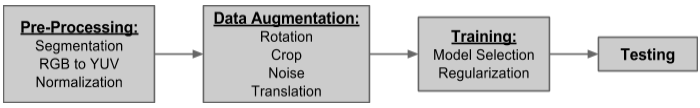
\includegraphics[width=9cm]{methodology}
\caption{Methodology}
\end{figure}

\subsection{Datasets}
\begin{description}
\item[IIIT hand gesture Dataset] \hfill
\begin{itemize}
  \item Train Images = 1100
  \item Test Images = 600
  \item Classes = 26
\end{itemize}
\item[Triesche Dataset] \hfill
\begin{itemize}
  \item Train Images = 600
  \item Test Images = 180
  \item Classes = 10
\end{itemize}
\end{description}

\subsection{Pre-Processing}
\subsubsection{Segmentation}  
The IIIT dataset contains images covering entire person but since we are interested in classification of hand gestures we have to segment the images to have just the hands as other portion of the image will be irrelevant and in most cases misleading for our task.
\begin{figure}[h]
\centering
\begin{subfigure}{.2\textwidth}
  \centering
  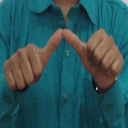
\includegraphics[width=.7\linewidth]{unsegmented}
  \caption{Unsegmented Image}
  \label{fig:sub1}
\end{subfigure}%
\begin{subfigure}{.2\textwidth}
  \centering
  
\includegraphics[width=.7\linewidth]{segmented}
  \caption{Segmented Image}
  \label{fig:sub2}
\end{subfigure}
\captionsetup{justification=centering}
\caption{Segmentation}
\label{fig:test}
\end{figure}

\subsubsection{RGB to YUV}
For the task of hand gesture recognition intensity variation is a better discriminative feature than chrominance. Since YUV images represent such intensity variation better than RGB images we have converted the images to YUV.

\subsubsection{Normalization}
If the dynamic range of one channel is very large while the dynamic range of other channels is relatively very low then the training will bias towards the larger dynamic range channels. In order to avoid such bias we have normalized the images per channel to the same range.

\subsection{Data Augmentation}
Since the number of training images are very less the classifier overfits training data very soon. So we have augmented the existing data using combination of 10° clockwise and counter-clockwise rotation, 5\% translation, addition of Gaussian and Salt \& Pepper noise and cropping, thereby increasing the training dataset size to 33, 000 images. By including such augmentations we hope that the trained model would be more robust to various real world effects like angle of camera, occlusions etc.\\
\begin{figure}[h]
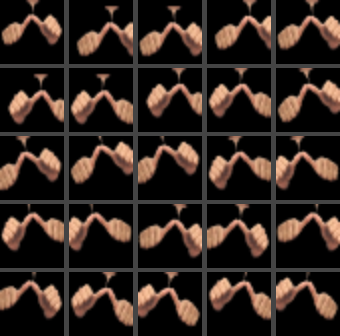
\includegraphics[width=9cm]{augmentedimages}
\caption{Augmented data}
\end{figure}
The easiest and most common method to reduce overfitting on image data is to artificially enlarge the dataset using label-preserving transformations. We employ four distinct forms of data augmentation, all of which allow transformed images to be produced from the original images with very little computation.

The form of data augmentation consists of generating image translations, rotations, scaling and noise. This increases the size of our training set by a factor of 30, though the resulting training examples are, of course, highly inter-dependent. Without this scheme, our network suffers from substantial overfitting, which would have forced us to use much smaller networks.

\subsection{Training}
In order to train a Convolutional neural network there a lot of parameters which can be optimized/tweaked based on the task to improve the performance. We have performed a lot of experiments training CNN by varying all such parameters like Convolution Kernel size, Pool size, Type of pooling, Image resolution, Optimization Algorithm, depth and width of convolutions, depth of MLP, type of activation functions, Regularization techniques like Dropout, Weight Decay and Normalization etc.
\begin{figure}[h]
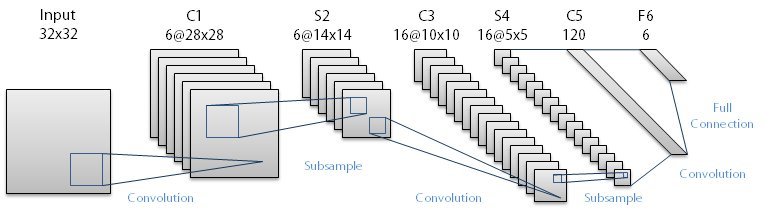
\includegraphics[width=9cm]{cnnarchitecture}
\caption{CNN Architecture}
\end{figure}

\subsubsection{Convolutional Neural Network}
Convolutional networks combine three architectural ideas to ensure some degree of shift and distortion invariance: local receptive elds, shared weights (or weight replication), and, sometimes, spatial or temporal subsampling. A typical convolutional network is shown in figure 4. The input plane receives images of characters that are approximately size-normalized and centered. Each unit of a layer receives inputs from a set of units located in a small neighborhood in the previous layer.

The idea of connecting units to local receptive fields on the input goes back to the Perceptron in the early 60s, and was almost simultaneous with Hubel and Wiesel's discovery of locally-sensitive, orientation-selective neurons in the cat's visual system. Local connections have been reused many times in neural models of visual learning. With local receptive elds, neurons can
extract elementary visual features such as oriented edges, end-points, corners (or similar features in speech spectrograms). These features are then combined by the higher layers. As stated earlier, distortions or shifts of the input can cause the position of salient features to vary.

In addition, elementary feature detectors that are useful on one part of the image
are likely to be useful across the entire image. This knowledge can be applied by forcing a set of units, whose receptive elds are located at different places on the image, to have identical weight vectors (Rumelhart, Hinton and Williams, 1986). The outputs of such a set of neurons constitute a feature map . At each position, different types of units in different
feature maps compute different types of features.

A sequential implementation of this, for each feature map, would be to scan the input image with a single neuron that has a local receptive field, and to store the states of this neuron at corresponding locations in the feature map. This operation is equivalent to a convolution with a small size kernel, followed by a squashing function. The process can be performed in parallel by implementing the feature map as a plane of neurons that share a single weight vector. Units in a feature map are constrained to perform the same operation on different parts of the image. A convolutional layer is usually composed of several feature maps (with different weight vectors), so that
multiple features can be extracted at each location.

The first hidden layer in figure 4 has 6 feature maps with 5 by 5 receptive fields. Shifting the input of a convolutional layer will shift the output, but will leave it unchanged otherwise. Once a feature has been detected, its exact location becomes less important, as long as its approximate position relative to other features is preserved. Therefore, each convolutional layer is followed by an additional layer which performs a local averaging and a subsampling, reducing the resolution of the feature map, and reducing the sensitivity of the output to shifts and distortions. The second hidden layer in figure 4 performs 2 by 2 averaging and subsampling, followed by a trainable
coefficient, a trainable bias, and a sigmoid. The trainable coefficient and bias control the effect of the squashing non-linearity (for example, if the coeffcient is small, then the neuron operates in a quasi-linear mode).

Successive layers of convolutions and subsampling are typically alternated, resulting in a "bi-pyramid" at each layer, the number of feature maps is increased as the spatial resolution is decreased. Each unit in the third hidden layer in figure 4 may have input connections from several feature maps in the previous layer.

Since all the weights are learned with back-propagation, convolutional networks can be seen as synthesizing their own feature extractor. The weight sharing technique has the inter-esting side effect of reducing the number of free parameters, thereby reducing the "capacity" of the machine and improving its generalization ability (see (LeCun, 1989) on weight sharing,
and learning and generalization for an explanation of notions of capacity and generalization). The network in figure 4 contains about 100,000 connections, but only about 2,600 free parameters because of the weight sharing. Such networks compare favorably with
other methods on handwritten character recognition tasks (Bottou et al., 1994), and they have been deployed in commercial applications.

\subsubsection{Dropout}
Combining the predictions of many different models is a very successful way to reduce test errors, but it appears to be too expensive for big neural networks that already take several days to train. There is, however, a very efficient version of model combination that only costs about a factor of two during training. The recently-introduced technique, called “dropout” [4], consists of setting to zero the output of each hidden neuron with probability 0.5. The neurons which are “dropped out” in this way do not contribute to the forward pass and do not participate in back-propagation. So every time an input is presented, the neural network samples a different architecture,but all these architectures share weights. This technique reduces complex co-adaptations of neurons, since a neuron cannot rely on the presence of particular other neurons. It is, therefore, forced to learn more robust features that are useful in conjunction with many different random subsets of the other neurons. At test time, we use all the neurons but multiply their outputs by 0.5, which is a reasonable approximation to taking the geometric mean of the predictive distributions produced by the exponentially-many dropout networks.

We use dropout in all the convolution layers. We did not notice any significant change either in classification accuracy or in speed of convergence by using dropout.

\subsubsection{Non-Linearities and Weight Normalization}
In traditional ConvNets this simply consists in a pointwise $tanh()$ sigmoid function applied to each site $(ijk)$. However, recent implementations have used more sophisticated non-linearities. A useful one for natural image recognition is the rectified sigmoid or $ReLU$:\\ 
\centerline{$R_{abs} : abs(g_i.tanh())$} \\ 
where $g_i$ is a trainable gain parameter. The rectified sigmoid is sometimes followed by a subtractive and divisive local normal-ization $N$, which enforces local competition between adjacent features in a feature map, and between features at the same spatial location. The subtractive normalization operation for a given site $x_{ijk}$ computes:\\ 
\centerline{$v_{ijk} = x_{ijk} − \sum_{ipq} w_{pq}.x_{i, j+p, k+q}$},\\ 
where $w_{pq}$ is a normalized truncated Gaussian weighting window (typically of size 9x9). The divisive normalization computes\\ \centerline{$y_{ijk}=v_{ijk} / max(mean(\sigma_{jk}), \sigma_{jk})$}\\ 
where $\sigma_{jk}=(\sum_{ipq} w_{pq}.v_{i, j+p, k+q}^2)^\frac{1}{2}$. The local contrast normalization layer is inspired by visual neuroscience models.

We observed that in our case $tanh()$ converges faster than $ReLU$. We also employed Local Contrastive Normalization for weights which slightly improves the classification accuracy.

\subsubsection{Feature Pooling Layer}
This layer treats each feature map separately. In its simplest instance, called
$P_A$, it computes the average values over a neighborhood in each feature map.
The neighborhoods are stepped by a stride larger than 1 (but smaller than or equal the pooling neighborhood). This
results in a reduced-resolution output feature map which is robust to small variations in the location of features in the
previous layer. The average operation is sometimes replacedby a max $P_M$. Traditional ConvNets use a pointwise
$tanh()$ after the pooling layer, but more recent models do not. Some ConvNets dispense with the separate pooling layer entirely
, but use strides larger than one in the filter bank layer to reducethe resolution. In some recent versions of ConvNets
,the pooling also pools similar feature at the same location, in addition to the same feature at nearby locations.
Supervised training is performed using a form of stochastic gradient descent to minimize the discrepancy between the
desired output and the actual output of the network. All the coefficient of all the filters in all the layers are updated
simultaneously by the learning procedure. The gradients are computed with the back-propagation method.

\subsection{Testing}
To avoid overfitting we have used the classification accuracy on test data after each epoch as the termination criterion.

\section{Experiments and Results}

% Please add the following required packages to your document preamble:
% \usepackage{graphicx}
\begin{table}[h]
\centering
\resizebox{.5\textwidth}{!}{%
\begin{tabular}{|c|c|c|c|p{3cm}|c|c|}
\hline
\multicolumn{1}{|l|}{\textbf{S.no}} & \multicolumn{1}{l|}{\textbf{Data}} & \multicolumn{1}{l|}{\textbf{Filter Size}} & \multicolumn{1}{l|}{\textbf{Pool Size}} & \multicolumn{1}{l|}{\textbf{Layers}}                                                                                     & \multicolumn{1}{l|}{\textbf{Train}} & \multicolumn{1}{l|}{\textbf{Test}} \\ \hline
1                                   & 1046x3x128x128                     & 5x5                                       & 2x2                                     & yuv(3x128x128)-\textgreater16x62x62-\textgreater256x29x29-\textgreater2-layered MLP(128-\textgreater26)                  & 100\%                               & 56\%                               \\ \hline
2                                   & 5230x3x128x128                     & 5x5                                       & 2x2                                     & yuv(3x128x128)-\textgreater16x62x62-\textgreater256x29x29-\textgreater2-layered MLP(128-\textgreater26)                  & 99\%                                & 55\%                               \\ \hline
3                                   & 5230x3x128x128                     & 31x31                                     & 2x2                                     & yuv(3x128x128)-\textgreater16x49x49-\textgreater256x9x9-\textgreater2-layered MLP(128-\textgreater26)                    & 87\%                                & 46\%                               \\ \hline
4                                   & 33000x3x64x64                      & 5x5                                       & 2x2                                     & yuv(3x64x64)-\textgreater16x30x30-\textgreater64x13x13-\textgreater256x4x4-\textgreater2-layered MLP(128-\textgreater26) & 99\%                                & 63\%                               \\ \hline
\end{tabular}
}
\caption{Experiments and Results on IIIT Database}
\label{my-label}
\end{table}
% Please add the following required packages to your document preamble:
% \usepackage{graphicx}

\begin{table}[h]
\centering
\resizebox{.5\textwidth}{!}{%
\begin{tabular}{|c|l|c|c|c|c|c|}
\hline
\multicolumn{1}{|l|}{\textbf{S.no}} & \textbf{Data}                                                                          & \multicolumn{1}{l|}{\textbf{Filter Size}} & \multicolumn{1}{l|}{\textbf{Pool Size}} & \multicolumn{1}{l|}{\textbf{Layers}}                                                                             & \multicolumn{1}{l|}{\textbf{Train}} & \multicolumn{1}{l|}{\textbf{Test}} \\ \hline
1                                   & \multicolumn{1}{c|}{75x1x64x64}                                                        & 5x5                                       & 2x2                                     & 1x64x64 -\textgreater 16x30x30 -\textgreater 64x13x13 -\textgreater 256x4x4 -\textgreater 128 -\textgreater 10   & 100\%                               & 76.6\%                             \\ \hline
2                                   & \multicolumn{1}{c|}{75x1x128x128}                                                      & 5x5                                       & 3x3                                     & 1x128x128 -\textgreater 16x41x41 -\textgreater 64x12x12 -\textgreater 256x2x2 -\textgreater 128 -\textgreater 10 & 99\%                                & 80\%                               \\ \hline
3                                   & \multicolumn{1}{c|}{\begin{tabular}[c]{@{}c@{}}75x1x128x128\\ with Sobel\end{tabular}} & 5x5                                       & 2x2                                     & 1x128x128 -\textgreater 16x41x41 -\textgreater 64x12x12 -\textgreater 256x2x2 -\textgreater 128 -\textgreater 10 & 100\%                               & 68\%                               \\ \hline
4                                   & \begin{tabular}[c]{@{}l@{}}75x1x128x128\\ + Sobel\\ + Dropout\\ + ReLU\end{tabular}    & 5x5                                       & 2x2                                     & 1x128x128 -\textgreater 16x41x41 -\textgreater 64x12x12 -\textgreater 256x2x2 -\textgreater 128 -\textgreater 10 & 99\%                                & 63\%                               \\ \hline
5                                   & \begin{tabular}[c]{@{}l@{}}75x1x128x128\\ +Sobel\\ +tanh\\ +Normalization\end{tabular} & 5x5                                       & 2x2                                     & 1x128x128 -\textgreater 16x41x41 -\textgreater 64x12x12 -\textgreater 256x2x2 -\textgreater 128 -\textgreater 10 & \multicolumn{1}{l|}{100\%}          & \multicolumn{1}{l|}{73.33\%}       \\ \hline
\end{tabular}
}
\caption{Experiments and Results on Triesch Database}
\label{my-label}
\end{table}

\subsection{Baseline Model}

Similar to terms in a text document, an image has local interest points or key points defined as salient image patches (small regions) that contain rich local information of the image. Keypoints are usually around the corners and edges of image objects, such as the edges of the map and around people’s faces. We use the Difference of Gaussian (DoG) detector [5] to automatically detect keypoints from images. The detected keypoints are depicted using PCA-SIFT descriptor, which is a 36-dimensional real-valued feature vector.
\begin{figure}[h]
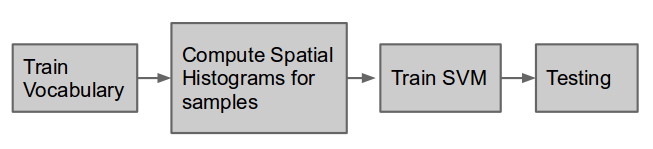
\includegraphics[width=9cm]{baseline}
\caption{Baseline Model}
\end{figure}
An image can be represented by a set of keypoint descriptors, but this set varies in cardinality and lacks meaningful ordering. This creates difficulties for many learning methods (e.g., supervised classifiers) that require feature vectors of fixed dimension as input. To address this problem, we use the vector quantization (VQ) technique which clusters the keypoint descriptors in their feature space into a large number of clusters using the K-means clustering algorithm and encodes each keypoint by the index of the cluster to which it belongs. We conceive each cluster as a visual word that represents a specific local pattern shared by the keypoints in that cluster. Thus, the clustering process generates a visual-word vocabulary describing different local patterns in images.  By mapping the key points to visual words, we can represent each image as a “bag of visual words”. This representation is analogous to the bag-of-words document representation in terms of form and semantics. Both representations are sparse and high-dimensional, and just as words convey meanings of a document, visual words reveal local patterns characteristic of the whole image.

SVM is used as the classifier for the different classes that are trained based on Bag of Visual words model.



\section{Conclusion}
Based on the analysis of various experiments we can conclude that data preprocessing,data augmentation helped in improving the classificaiton accuracy. Model parameters such as depth of convolution, number of feature maps per layer,Convolution Kernel size, Pool size need to be adjusted such that each unit in the last convolution layer would have a receptive field of atleast $80\%$ of the input image. Regularization techniques such as Dropout, Weight Decay has only improved the classification accuracy by negligible factors. Compared with the baseline model the accuracy has improved by two folds by using CNN for classfication. Although CNN gave very good results for some classes the model gave mixed results for similar looking hand gestures like for M and N.



\section*{Acknowledgment}


The authors would like to thank Ridhiman Dasgupta for the insightful discussions and for his help in providing infrastructure for running experiments.





% trigger a \newpage just before the given reference
% number - used to balance the columns on the last page
% adjust value as needed - may need to be readjusted if
% the document is modified later
%\IEEEtriggeratref{8}
% The "triggered" command can be changed if desired:
%\IEEEtriggercmd{\enlargethispage{-5in}}

% references section

% can use a bibliography generated by BibTeX as a .bbl file
% BibTeX documentation can be easily obtained at:
% http://www.ctan.org/tex-archive/biblio/bibtex/contrib/doc/
% The IEEEtran BibTeX style support page is at:
% http://www.michaelshell.org/tex/ieeetran/bibtex/
%\bibliographystyle{IEEEtran}
% argument is your BibTeX string definitions and bibliography database(s)
%\bibliography{IEEEabrv,../bib/paper}
%
% <OR> manually copy in the resultant .bbl file
% set second argument of \begin to the number of references
% (used to reserve space for the reference number labels box)
\begin{thebibliography}{1}

\bibitem{IEEEhowto:kopka}
Jmaa, A.B., Mahdi, W., Jemaa, Y.B., Hamadou, A.B.: Hand localization and fingers features extraction: Application to digit recognition in sign language. In: Corchado, E., Yin, H. (eds.) IDEAL 2009. LNCS, vol. 5788, pp. 151–159. Springer, Heidelberg (2009)

\bibitem{IEEEhowto:kopka}
Lecun, Y., Bottou, L., Bengio, Y., Haffner, P.: Gradient-based learning applied to document recognition. Proceedings of the IEEE, 2278–2324 (1998)

\bibitem{IEEEhowto:kopka}
Nagi, J., Ducatelle, F., Di Caro, G., Ciresan, D., Meier, U., Giusti, A., Nagi, F.,
Schmidhuber, J., Gambardella, L.: Max-pooling convolutional neural networks for
vision-based hand gesture recognition. In: IEEE International Conference on Signal
and Image Processing Applications (ICSIPA), pp. 342–347 (2011)

\bibitem{IEEEhowto:kopka}
G.E. Hinton, N. Srivastava, A. Krizhevsky, I. Sutskever, and R.R. Salakhutdinov. Improving neural net-
works by preventing co-adaptation of feature detectors.
arXiv preprint arXiv:1207.0580
, 2012.

\bibitem{IEEEhowto:kopka}
D. G. Lowe. Distinctive image features from scale-invariant keypoints. Int. J. Comput. Vision, 60(2):91–110, 2004.
  
\end{thebibliography}




% that's all folks
\end{document}


